   
        
        \begin{ledgroupsized}[r]{120mm}
        \footnotesize 
        \pstart        
        \noindent\textbf{\"{U}berlieferung:}  
        \pend
        \end{ledgroupsized}
      
       
              \begin{ledgroupsized}[r]{114mm}
              \footnotesize 
              \pstart \parindent -6mm
              \makebox[6mm][l]{\textit{L}}Konzept: LH XXXVII 2 Bl. 1\textendash 2. 1 Bog. 2\textsuperscript{o}. 1 S. zweispaltig auf Bl. 1 r\textsuperscript{o}. Linke Spalte fortlaufender Text, rechts in der Mitte die Zeichnung \textit{[Fig. 1]}. Die verbleibenden Seiten des Bogens N. 15 und N. 16.\pend
              \end{ledgroupsized}
       
              \begin{ledgroupsized}[r]{114mm}
              \footnotesize 
              \pstart \parindent -6mm
              \makebox[6mm][l]{\textit{E}}\cite{00243}\textsc{Gerland} 1906, S.~89f.\\KK 1, Nr. 973 A\pend
              \end{ledgroupsized}
        %\normalsize
        \vspace*{5mm}
        \begin{ledgroup}
        \footnotesize 
        \pstart
      \noindent\footnotesize{\textbf{Datierungsgr\"{u}nde}: Der Texttr\"{a}ger des vorliegenden St\"{u}cks ist Papier der Zeit vor Leibniz' Parisaufenthalt. Die genauere Datierung erfolgt aufgrund des Wasserzeichens, das in \textit{LSB} VI, 2, N. 45, 46 und 48 belegt ist. Wir \"{u}bernehmen die 2. H\"{a}lfte 1671 als Entstehungszeit unseres St\"{u}cks.}
        \pend
        \end{ledgroup}
      
        \vspace*{8mm}
        \pstart 
        \normalsize
  \centering [1 r\textsuperscript{o}] Problemata Optica Nova\\ reperta a\\ G. G. \protect\edlabel{ponrstart}L. L.\pend \vspace{1.0ex} \pstart \textso{Probl. 1.} Efficere ut omnes radii a quolibet puncto dato objecti dati ducti ad puncta superficiei objectivae aequidistantia a puncto dato colligantur in unum punctum. \pend \pstart \centering\protect\textso{Solutio:} \pend \vspace{1.0ex}
  \pstart Efficietur hoc: si omnes superficies refringentes sint sphaericae concentricae, et faciant radios \protect\edlabel{ponrend}\edtext{convergentes.}{{\xxref{ponrstart}{ponrend}}\lemma{L. L.}\Afootnote{\textit{ (1) }\ Probl. 1. Omnes radios unius \textbar\ cujuslibet \textit{ erg.}\ \textbar\ puncti objecti dati colligere in unam lineam, per refractionem\protect\index{Sachverzeichnis}{refractio|textit}, ita ut radii omnes a dato puncto ad superficiem refringentem objectivam.  Si omnes superficies refringentes sint sphaericae concentricae; faciantque radios convergentes: radii omnes unius puncti \textit{ (2) }\ \textso{Probl.} [...] refringentes sint  \textbar\ sphaericae \textit{ erg.}\ \textbar\ concentricae, et faciant radios convergentes. \textit{ L}}} \pend \newpage
     \begin{center}
     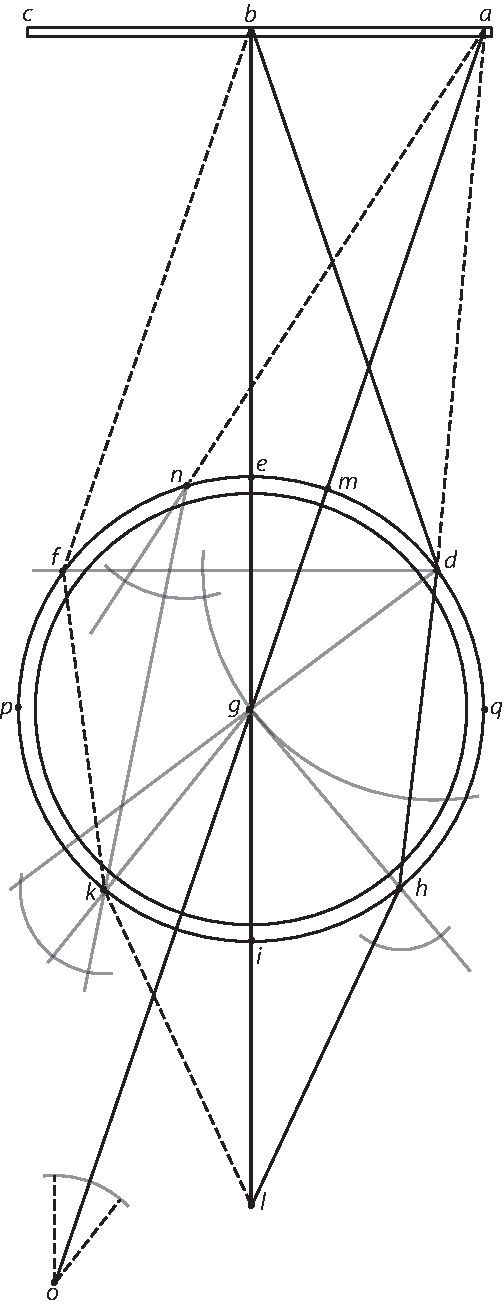
\includegraphics[width=0.37\textheight]{images/37_2_1r}\\
     \hspace{1mm} \textit{[Fig. 1, tlw. Blindzeichnung]}
     \end{center}
\pstart \centering\textso{Demonstratio} \pend \vspace{1.0ex}\pstart 
Esto objectum \textit{abc} Superficies refringens sphaerica objectiva \textit{def} cujus centrum \textit{g} puncti \textit{b} radius perpendicularis refractionis \protect\index{Sachverzeichnis}{refractio} expers \textit{beg} continuetur ultra \textit{g}. Radius \textit{bd} refractus in \textit{d} ad perpendicularem \edtext{in medium densius ex rariore}{\lemma{}\Afootnote{in medium densius ex rariore \textit{ erg.} \textit{ L}}} versus \textit{h} incidat in \textit{h} in aliam superficiem sphaericam \textit{hik} superficiei \textit{def} concentricam; per quam rursus in medium rarius egrediatur. Ne igitur divergat radius \textit{bdh} ab irrefracto \textit{beg} continuato; patet superficiem \textit{hik} debere concavitatem obvertere medio densiori. Ita radius \textit{bdh} secabit radium \textit{beg} in \textit{l}. Eodem modo radius \textit{bf} refractus\edtext{}{\lemma{}\Afootnote{refractus \textbar\ ad \textit{ streicht Hrsg.}\ \textbar\ in \textit{ L}}} in medium densius ad \textit{k} ex densiore refringetur ad \textit{l}. Idemque dicendum est de omnibus punctis superficiei \textit{def} \edtext{distantibus}{\lemma{\textit{def}}\Afootnote{ \textit{ (1) }\ aequidistantibus \textit{ (2) }\ distantibus \textit{ L}}} a puncto \textit{b} quantum ab eo distat punctum \textit{d}. Id est qui continentur circumferentia circuli in superficie sphaerica cujus diameter est \textit{df}.\pend \pstart Idem dicendum de radiis \textit{ad}, \textit{an} et omnibus aliis in plano non designabilibus qui continentur circumferentia circuli in superficie sphaerica, cujus diameter \textit{dn}. Colligentur enim omnes in  puncto \textit{o}. \pend \pstart Observandum est nihil referre sive superficies \textit{def} et \textit{hik} sint portiones ejusdem sphaerae, sive sphaerarum concentricarum. Posse item vel adhiberi vel corpus cylindricum \textit{def}, \textit{kih} contentum superficiebus sphaericis \textit{def}, \textit{hik} et \edtext{planis}{\lemma{et}\Afootnote{ \textit{ (1) }\ rectis \textit{ (2) }\ planis \textit{ L}}} \textit{dh}, \textit{fk} vel sphaeram integram \textit{defpkih}. \pend 